% ---- Modele TP PC V2 -----------
\documentclass[a4paper,10pt,french]{scrartcl}
\usepackage[T1]{fontenc}%---pour l'encodage d'entr\'ee
\usepackage{array}%---pour les tableaux
\usepackage{titlesec}%---modification des titres
\usepackage{ulem}%---pour le soulignage
\usepackage[dvipsnames]{xcolor}%---pour avoir d'autres couleurs
\usepackage{color}%---pour avoir les couleurs de base
\usepackage{babel}%---pour les trucs de langue et la francisation

\usepackage{graphicx}%----pour mettre des images
\usepackage[utf8]{inputenc}%---encodage
\usepackage{geometry}%---pour modifier les tailles et mettre a4paper
%\usepackage{awesomebox}%---pour les boites d'exercices, de pbq et de croquis ---d\'esactiv\'e pour les TP de PC
\usepackage{tikz}%---pour dessiner + d\'ependance de chemfig
%\usepackage{tabularx}%---pour dimensionner automatiquement les tableaux avec variable X
\usepackage{fancyhdr}%---pour les en-t\^ete personnalis\'ees
\usepackage{blindtext}%---pour les liens
\usepackage{hyperref}%---pour les liens (\`a mettre en dernier)
\usepackage{caption}%---pour la francisation de la l\'egende table vers Tableau
 \usepackage{float}% --- pour placer les figures et tableaux où l'on souhaite avec argument H

\captionsetup{labelfont=sc}%---pour la francisation de la l\'egende table vers Tableau
\def\frenchtablename{Tableau}%---pour la francisation de la l\'egende table vers Tableau
\pagestyle{fancy}
\renewcommand\headrulewidth{1pt}
\fancyhead[L]{TP n°4}
\fancyhead[R]{Saux - Gadré-Dacheville}
\title{Compte rendu de TP N°4}
\date{}
\author{}

\geometry{a4paper}
% ----------- Création des commandes de couleur ----------
\makeatletter
\newcommand{\coloruline}[2]{%
        \UL@protected\def\temp@uline{\leavevmode \bgroup
            \markoverwith{\textcolor{#1}{\rule[-0.5ex]{2pt}{0.4pt}}}%
        \ULon}%
        \temp@uline{#2}%
    }

    \newcommand{\coloruuline}[2]{%
        \UL@protected\def\temp@uuline{\leavevmode \bgroup
            \UL@setULdepth
            \ifx\UL@on\UL@onin \advance\ULdepth2.8\p@\fi
            \markoverwith{\textcolor{#1}{\lower\ULdepth\hbox
                {\kern-.03em\vbox{\hrule width.2em\kern1\p@\hrule}\kern-.03em}}}%
        \ULon}%
        \temp@uuline{#2}%
    }

\makeatother

\renewcommand{\thesection}{\arabic{section}}
\renewcommand{\thesubsection}{\arabic{subsection}}
\renewcommand{\thesubsubsection}{\arabic{subsubsection}}
\begin{document}
% ---------------- Modification des titres de niveau 1,2 et 3 --------------------
\titleformat
{\section} % command
%[display] % shape
{\Large} % format
{\coloruuline{red}{\thesection. }} % label
{0ex} % sep
{\coloruuline{red}} % before-code
[] % after-code

\titleformat
{\subsection} % command
%[display] % shape
{\Large} % format
{\coloruline{red}{\thesection.\thesubsection. }} % label
{0ex} % sep
{\coloruline{red}} % before-code
[] % after-code

\titleformat
{\subsubsection} % command
%[display] % shape
{\large} % format
{\coloruline{ForestGreen}{\thesection.\thesubsection.\thesubsubsection. }} % label
{0ex} % sep
{\coloruline{ForestGreen}} % before-code
[] % after-code

\titleformat
{\chapter} % command
%[display] % shape
{\large} % format
{\coloruline{NavyBlue}{\thechapter \:- }} % label
{0ex} % sep
{\coloruline{NavyBlue}} % before-code
[] % after-code


% ---------------- Début du corps du document ------------------------------------

\section{Introduction}
L'objectif de ce TP est d'étudier l'isochronisme des oscillations d'un pendule, puis de mesurer l'intensité de pesanteur \(g\) à Toulouse puis sur d'autres planètes. La première partie nous permettra de déterminer l'angle d'amplitude avec lequel effectuer les mesures pour déterminer \(g\). La seconde partie du TP se concentrera sur la mesure de \(g\) à  Toulouse et la dernière partie sur la détermiation de l'intensité de pesanteur d'autres planèes.
\section{Protocole}
Nous allons effectuer trois manipulations dinstinctes, une pour chaque partie du TP.
\subsection{Isochronisme des oscillations}
\subsubsection{Matériel}
\begin{itemize}
 \item Un pendule constitué d'une tige de longueur 30cm et d'une masse située à une distance variable.
 \item Un capteur eu U
 \item Une carte d'acquisition SYSAM-SP5
 \item Trois fils électriques
\end{itemize}
\subsubsection{Description du montage expérimental}
\begin{figure}[H]
\begin{center}
 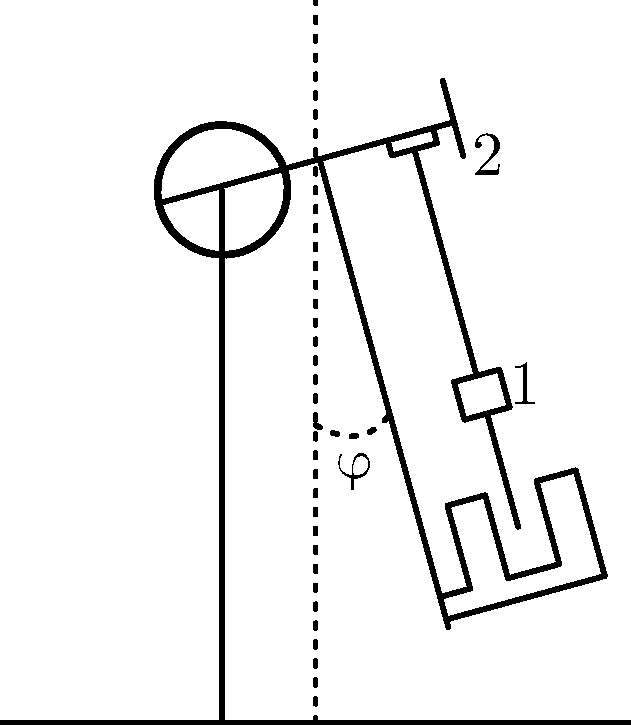
\includegraphics[scale=0.5]{schema}
 \end{center}
\end{figure}

Nous fixons la masse (1) sur la tige à une longueur \(l\) de l'origine de la tige, réglons l'amplitude d'oscillation \(\theta\) à l'aide du disque gradué (2) et l'inclinaison du pendule \(\varphi\).
\subsubsection{Mesures à effectuer}
\begin{enumerate}
 \item Fixer une longueur \(l = 25 cm\)
 \item Régler les paramètres d'acquisition de LATIS-PRO sur un temps d'acquisition de 10s, Un intervalle de mesure de 2 ms, un nombre de points de 6500.
 \item Lacher le pendule avec une amplitude de \(\theta = 5°\) et commencer l'enregistrement
 \item Avec l'outil réticule libre de LATIS-PRO, mesurer le premier l'abiscice du premier pic et du 20e pic
 \item Répéter les étapes 3 et 4 cinq fois.
 \item Répéter les étapes 3 et 4 en faisant varier \(\theta\) jusquà \(90°\) par pas de \(5°\).
\end{enumerate}
\subsection{Mesure de l'intensité de pesanteur terrestre}
\subsubsection{Matériel et description du montage expérimental}
Il s'agit du m\^eme montage expérimental que dans la partie précédente.
\subsubsection{Mesures à effectuer}
\begin{enumerate}
 \item Fixer une longueur \(l = 5 cm\)
 \item Régler les paramètres d'acquisition de LATIS-PRO sur un temps d'acquisition de 10s, Un intervalle de mesure de 2 ms, un nombre de points de 6500.
 \item Lacher le pendule avec une amplitude de \(\theta = 25°\) et commencer l'enregistrement
 \item Avec l'outil réticule libre de LATIS-PRO, mesurer le premier l'abiscice du premier pic et du 20e pic
 \item Répéter les étapes 3 et 4 en faisant varier \(l\) jusquà \(25\) cm par pas de \(5\) cm.
\end{enumerate}
\subsection{Mesure de l'intensité de pesanteur d'autres planètes}
\subsubsection{Matériel et description du montage expérimental}
Il s'agit du m\^eme montage expérimental que dans la partie précédente.
\subsubsection{Mesures à effectuer}
\begin{enumerate}
 \item Fixer une longueur \(l = 25 cm\)
 \item Régler les paramètres d'acquisition de LATIS-PRO sur un temps d'acquisition de 10s, Un intervalle de mesure de 2 ms, un nombre de points de 6500.
 \item Régler l'inclinaison \(\varphi\) du pendule sur \(10°\)
 \item Lacher le pendule avec une amplitude de \(\theta = 5°\) et commencer l'enregistrement
 \item Avec l'outil réticule libre de LATIS-PRO, mesurer le premier l'abiscice du premier pic et du 20e pic
 \item Répéter les étapes 3 à 5 en faisant varier \(\varphi\) jusquà \(80°\) par pas de \(10°\).
\end{enumerate}
\section{Mesures}
\subsection{Isochronisme des oscillations}
\subsubsection{Données}
\begin{table}[H]
\begin{center}
\begin{tabular}{ll}
Mesure & Période (s)\\
1 & 0.9846\\
2 & 1.0068\\
3 & 1.0079\\
4 & 1.01\\
5 & 1.0068\\
6 & 1.0054
\end{tabular}
\end{center}
\caption{Mesure de la période T avec un angle de 5°}
\end{table}

\begin{table}[H]
\begin{center}
\begin{tabular}{ll}
Amplitude (°) & Période (s)\\
10 & 1.009\\
15 & 1.0111\\
20 & 1.0165\\
25 & 1.0186\\
30 & 1.0219\\
35 & 1.0304\\
40&1.0347\\
45&1.0412\\
50&1.053\\
55&1.0606\\
60&1.0734\\
65&1.0831\\
70&1.0905\\
75&1.1077\\
80&1.1174\\
85&1.1356\\
90&1.1593
\end{tabular}
\end{center}
\caption{Mesure de la période T en fonction de l'amplitude}
\end{table}
\subsubsection{Incertitude}
La période est soumise aux deux types d'incertitude.

La période pour 10 oscillations est obtenue en faisant la différence entre le temps pour obtenir le premier pic et le temps pour obtenir le 20 eme pic. L'incertitude d'un de ces temps est lié à la précision de LATIS-PRO, qui est de 1 ms ou 0.001s. L'incertitude de type B pour une période est alors de \[\frac{\frac{0.001}{\sqrt{3}} + \frac{0.001}{\sqrt{3}}}{10} = 1.15\cdot 10^{-4} s\]

Nous avons effectué  6 mesures. L'incertitude de type A liées à ces mesures est donnée par \[u_A(T_0) = \frac{\sigma}{\sqrt{N}}\] avec \[\sigma = \sqrt{\frac{1}{5}\sum^{6}_{i=1}(T_i-\bar{T})^2} = 9.383\cdot10^{-3} s\] et \[\bar{T} = \frac{1}{5}\sum^6_{i=1} T_i\]

L'incertitude finale sur la période est donc de  \[\sqrt{u^2_A(T)+u^2_B(T)} = \sqrt{\frac{(9.383\cdot10^{-3})^2}{6} + (1.15\cdot 10^{-4})^2 } = 3.83\cdot 10^{-3} s\]

Pour \(\theta = 5°\), on obtient donc \(T = (1.00\pm 3.83\cdot 10^{-3})s\).

L'incertitude liée à l'angle est uniquement de type B. Il faut prendre en compte la gradution di disque gradué, qui sert de repère pour placer la tiger, mais aussi la largeur de la tige, qui empeche de la placer exactement sur la bonne graduation. On estime que l'incertitude liée à la graduation est négligeable par rapport à celle liée à la largeur de la tige. On estime cette incertitude à environ 3°. De plus, le 0 du disque gradué n'était pas correctement étalonné. Il a fallu le placer avant de commencer les manipulations pour qu'il corresponde à la position verticale de la tige. On estime cette erreur à environ 1°. Cette erreur est systématique et va donc s'appliquer à toutes les mesures d'angle.

L'incertitude de type B pour chaque angle est donc de \(1+3 = 4\)°.
\subsection{Mesure de la pesanteur terrestre}
\subsubsection{Données}
\begin{table}[H]
\begin{center}
\begin{tabular}{ll}
Longueur (cm) & Période (s)\\
5 & 0.664\\
10 & 0.722\\
15 & 0.819\\
20 & 0.921\\
25 & 1.013
\end{tabular}
\end{center}
\caption{Mesure de la période T en fonction de la longueur de tige avec une amplitude de 25°}
\end{table}
\subsubsection{Incertitude}
l'incertitude liée à la longueur de tige \(l\) est uniquement de type B. Elle est produite par la précision de la graduation mais aussi par la hauteur de la masse coulissante. On estime que l'erreur liée à la graduation est négligeable devant la hauteur de la masse, qui empeche de placer avec précision le milieu de la masse à la hauteur de tige souhaitée. On estime cette incertitude à environ 5mm.

L'incertitude liée à la période est la m\^eme que dans la partie précédente, c'est à dire de \(3.83\cdot 10^{-3}\) s

L'incertitude sur l'angle d'amplitude est la m\^eme que dans la partie précédente, c'est à dire de \(4\)°.
\subsection{Mesure de l'intensité de pesanteur d'autres planètes}
\subsubsection{Données}
\begin{table}[H]
\begin{center}
\begin{tabular}{ll}
Angle (°) & Période (s)\\
10 & 1.0195\\
20 & 1.043\\
30 & 1.086\\
40&1.148\\
50&1.241\\
60&1.404\\
70&1.695\\
80&2.314
\end{tabular}
\end{center}
\caption{Mesure de la période T en fonction de l'inclinaison du pendule pour une amplitude de 5°}
\label{tab:inclinaison}
\end{table}
\subsubsection{Incertitude}
L'incertitude liée à la période est la m\^eme que dans la partie précédente, c'est à dire de \(3.83\cdot 10^{-3}\) s

L'incertitude sur l'angle d'amplitude est la m\^eme que dans la partie précédente, c'est à dire de \(4\)°.

L'incertitude liée sur l'inclinaison du pendule est uniquement de type B. Elle est produite par le système permettant de maintenir le pendule à l'inclinaison choisie. Il faut prendre en compte l'incertitude liée à la graduation du disque permettant de mesure l'angle d'inclinaison mais aussi la façon dont le pendule est maintenu dans la position. La pièce rentrant dans le trou de fixation étant de diamètre inférieur au trou, on observe un décalage de l'ordre du degré selon la position de la pièce dans le trou. L'incertitude liée à l'inclinaison du pendule est donc de \[\frac{1}{\sqrt{3}}+ 1 = 1.58 \texttt{°}\]
\section{Graphiques}
\begin{figure}[H]
\begin{center}
 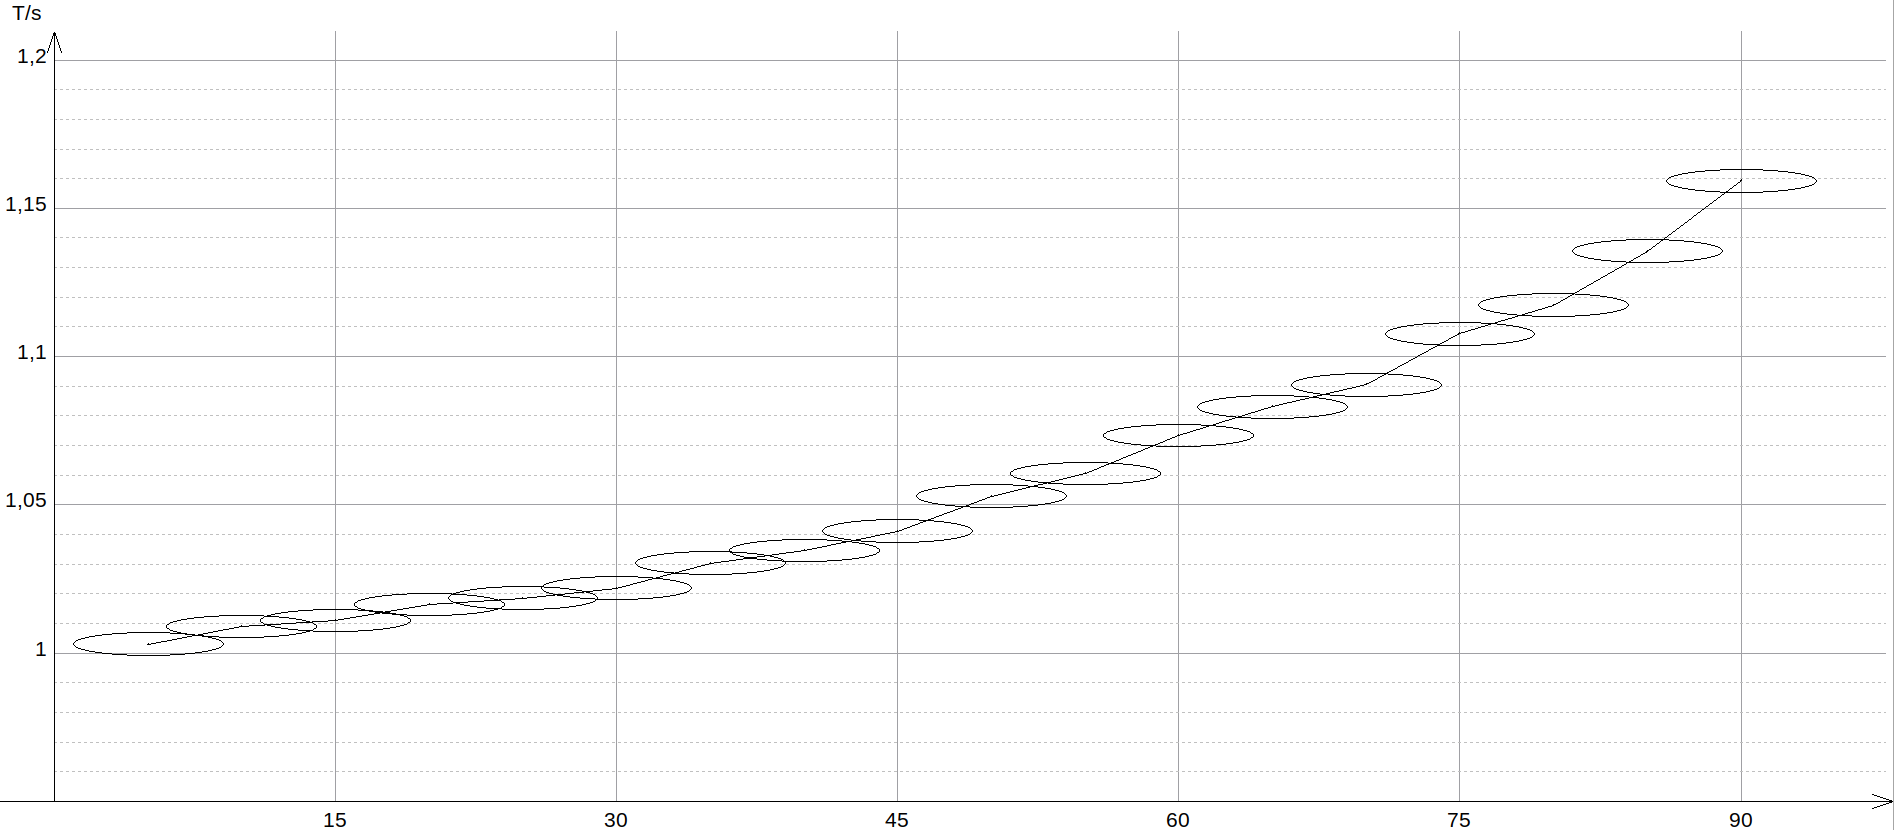
\includegraphics[scale=0.3]{graph_1}
 \end{center}
 \caption{Évolution de la période (s) en fonction de l'amplitude (°)}
\end{figure}
\begin{figure}[H]
 \begin{center}
 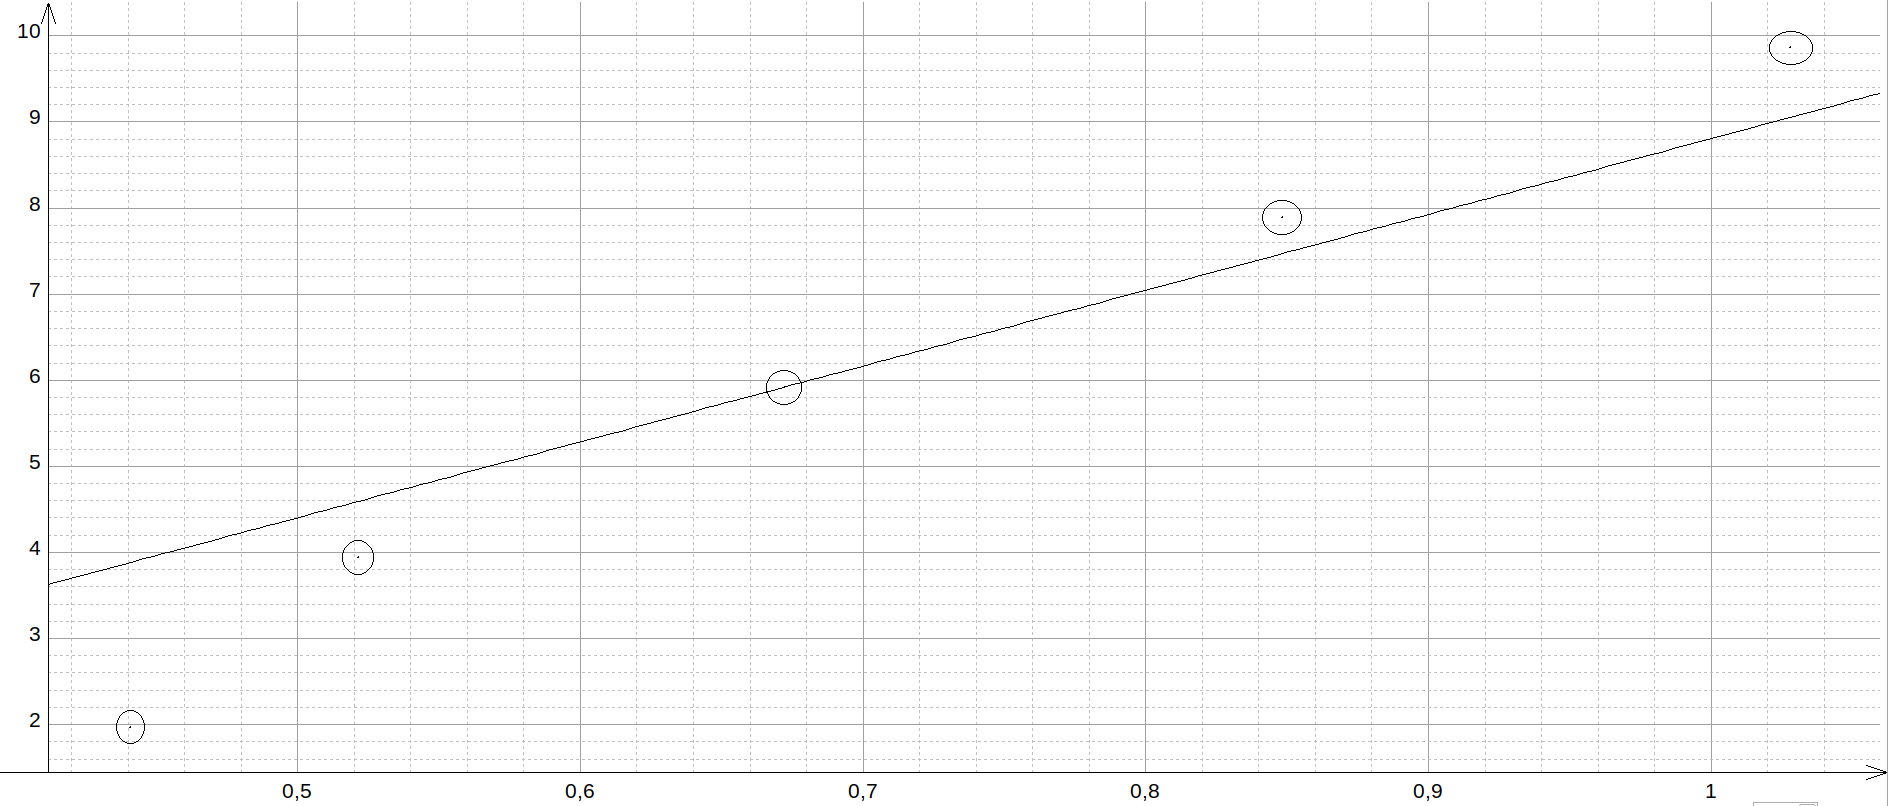
\includegraphics[scale=0.3]{graph_2}
 \end{center}
 \caption{Évolution de \(4\pi^2l\) en fonction de la période au carré \(T^2\). Dans cette modélisation, \(g\)  est la pente de la droite.}
\end{figure}
\begin{figure}[H]
 \begin{center}
 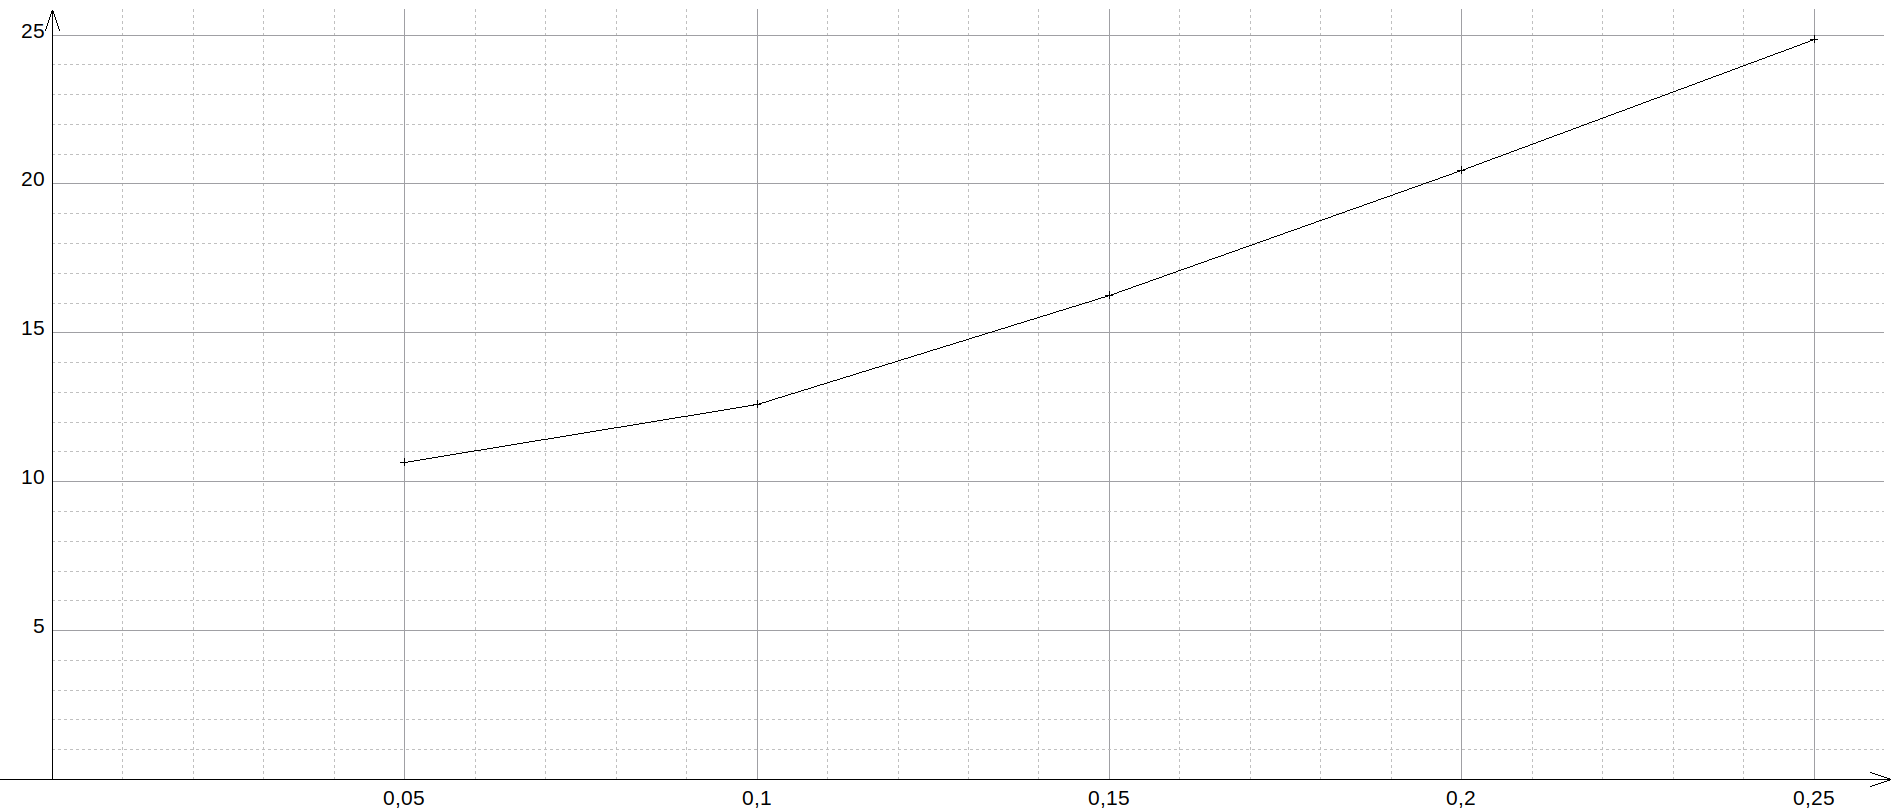
\includegraphics[scale=0.3]{graph_3}
 \end{center}
 \caption{Évolution de longueur corrigée L en fonction de la longueur effective l. On recherche la valeur de l telle que \(L = f(l)\).}
\end{figure}
\begin{figure}[H]
 \begin{center}
 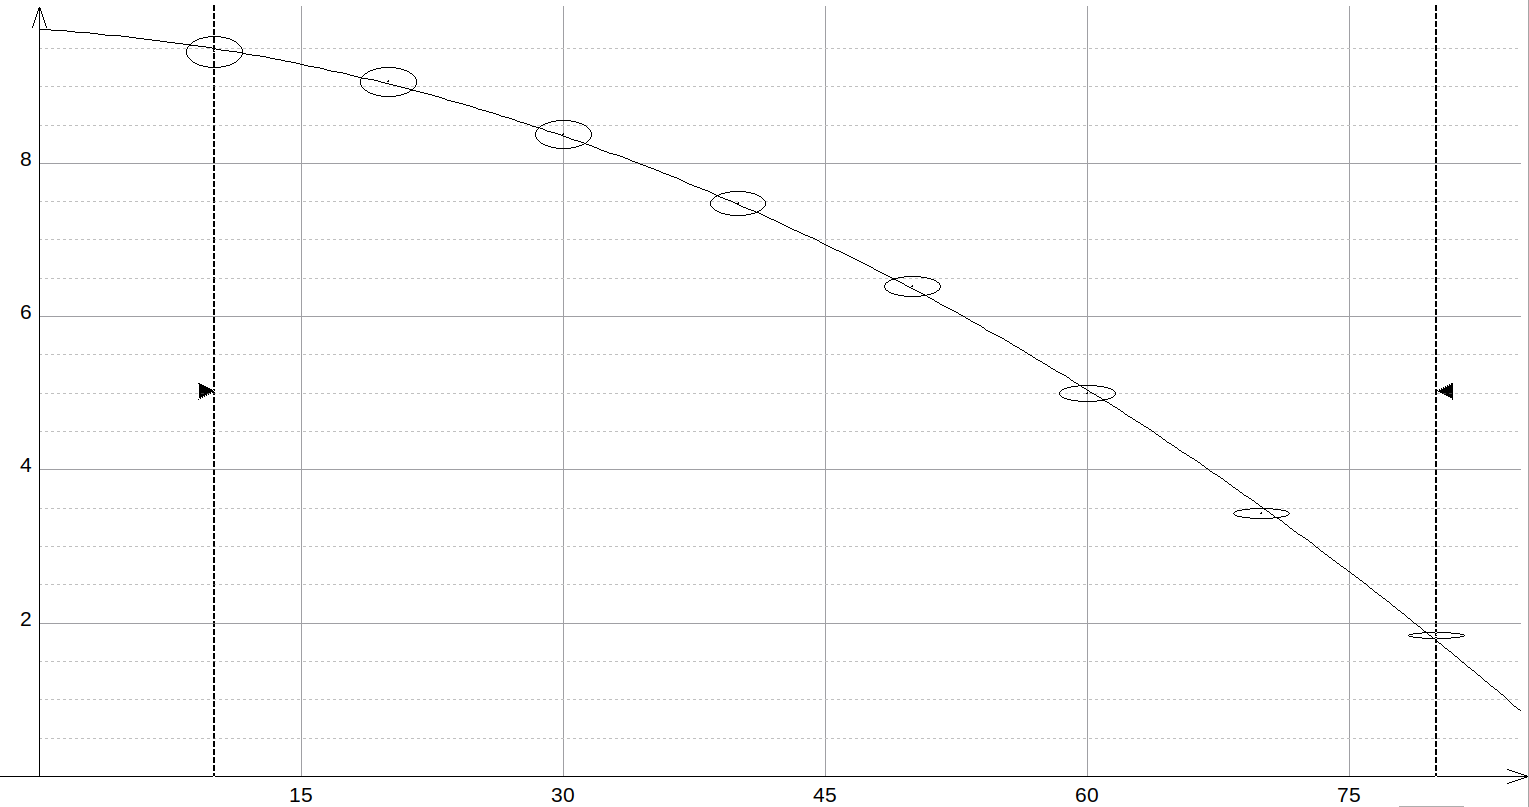
\includegraphics[scale=0.3]{graph_4}
 \end{center}
 \caption{Évolution de \(g_e\) l'intensité de pesanteur simulée en fonction de l'angle d'inclinaison \(\varphi\) }
\end{figure}
\section{Exploitation des résultats}
\subsection{Isochronisme des oscillations}
Pour un angle \(\theta\) de 5°, la valeur moyenne obtenue est de 1.003 s avec une incertitude \(u\) de \(3.83\cdot 10^{-3}\) s. Pour obtenir un niveau de confiance de 95\%, il faut multiplier \(u\) par 2. La valeur obtenir avec ce taux de confiance est donc de \(1.00\pm 7.66 \cdot10^{-3}\)s.

En traçant \(T(\theta)\), on remarque que l'amplitude des valeurs prises pour des angles jusqu'à 25° est inférieure à 0.2s. Compte tenu des incertitudes de \(7.66 \cdot10^{-3}\) pour un indice de confiance de 95\%, on peut considérer qu'il y a isochronisme jusqu'à cet angle. À partr de 30°, l'évolution de la période est trop rapide, et m\^eme en considérant l'incertitude, on atteint des écarts trop importants.

Afin de diminuer l'incertitude relative sur l'angle d'amplitude, on prendra dans la suite du TP l'angle le plus grand où l'on considère qu'il y a isochronisme, i.e 25°.
\subsection{Mesure de la pesanteur terrestre}
Pour un pendule dont on néglige les forces de frottement, avec des angles d'oscillation faibles, on peut définir la période d'oscillation comme : \begin{equation}T = 2\pi \frac{l}{g}\label{eq:1}\end{equation} À partir de cette expression, on peut obtenir g en traçant \[4\pi^2l = f(T^2)\] On devrait obtenir une droite, dont la pente sera la valeur de \(g\).

On obtient une pente de \((8,81 \pm 0,67) m \cdot s^{-2}\) pour un intervalle de confiance de 95\%. M\^eme en considérant les incertitudes, cette valeur est trop éloignée de la valeur attendue. On a en effet un écart de \(\frac{9.81-8.81}{9.81} *100 = 10.1\% \) qui ne s'explique pas par un problème expérimental. Il s'agit d'une erreur de modélisation. On en effet considéré la tige du pendule sans masse et la masse sans volume (en plus de négliger les forces de frottements solides entre la tige et son support et fluides avec l'air).

On peut corriger la modélisation en considérant en déterminant la longueur \(l = L\) avec \(L = g_e\times \frac{T^2}{4\pi^2}\). Pour ce faire, on va tracer avec regressi \(L = f(l)\) pour trouver ce point.

La longueur la plus proche de cette condition est celle de 25 cm.

En prenant uniquement, \(l = 25\)cm, on peut déterminer g. En effet, on déduit de \ref{eq:1} que \[g = \frac{4\pi^2l}{T^2} = 9.61 m\cdot s^{-2}\]

L'incertitude de cette valeur est \[u(g) = \sqrt{(\frac{u(l)}{l})^2+(\frac{u(T)}{T})^2} \times g = \sqrt{(\frac{0.005}{0.25})^2+(\frac{3.83\cdot10^{-3}}{1.013})^2}\times 9.61 = 0.195 \]

Ainsi, avec un indice de confiance de 95\%, \[g = (9.61\pm 0.39 )m\cdot s^{-2}\]

Cette valeur est plus cohérente que la précente ; la valeur de référence se trouve dans l'intervalle trouvé. Il s'agissait bien d'une erreur de modélisation du pendule. Pour les prochaines mesure, on utilisera une longueur \(l = 25\)cm.
\subsection{Mesure de la pesanteur sur d'autres planètes}
L'objectif est de déterminer l'influence de la mesure du temps pour des astronautes sur la Lune et sur Mars s'ils mesuraient le temps avec un pendule.

En inclinant le pendule d'un angle \(\varphi\), on peut modifier la valeur du poids qui affecte la masse en le multipliant par \(\cos(\varphi)\).

On peut alors écrire la période comme
\begin{equation}
T = 2\pi \frac{l}{g\cos(\varphi)}
\end{equation}

On va d'abord trouver quelle valeur d'angle il faut pour simuler la pesanteur sur les deux astres. Pour ce faire, on va établir une relation entre \(g_e\) et \(\cos(\varphi)\). On va donc calculer pour chaque valeur d'angle d'inclinaison l'intensité de pesanteur simulée avec \[g_e = \frac{4\pi^2 l}{T^2}\] et la tracer en fonction de \(\varphi\).

On peut vérifier que les valeurs trouvée expérimentalement de  \(g_e\) sont cohérentes en les comparant avec les valeurs théoriques \(g_{e,th} = g_{Terre}\times \cos(\varphi)\).

Pour modéliser expérimentalement la relation entre \(g_e\) et \(\varphi\), la fonction qui semble le mieux correspondre est une fonction du second degrés. Ce n'est pas étonnant car la fonction parabolique est la fonction disponible dans Regressi qui se rapproche le plus de la fonction cosinus.

Régressi modélise la fonction comme \[g_e = a+b\varphi+c\varphi^2\]
avec \(a =( 9,749 \pm 0,085), b = (-14,5 \pm 4,3), c = (-1,065 \pm 0,047)\)

On peut maintenant déterminer la période d'un pendule sur la Lune et Mars. On sait que \(g_{Lune} = 0.166g_{Terre} \Rightarrow \cos(\varphi) = 0.166 \Rightarrow \varphi = 80°\). De plus, \(g_{Mars} = 0.38g_{Terre} \Rightarrow \cos(\varphi) = 0.38 \Rightarrow \varphi = 68°\)

Sur Mars (\(\varphi \simeq 70\)°), d'après le tableau \ref{tab:inclinaison}, on trouve une période de \(1.695 \pm 0.0038\) s, ce qui signifie que le temps mesuré uniquement avec le pendule passe 1.7 fois plus lentement que sur Terre.

Sur la Lune (\(\varphi \simeq 80\)°), d'après le tableau \ref{tab:inclinaison}, on trouve une période de \(2.314 \pm 0.0038\) s, ce qui signifie que le temps mesuré uniquement avec le pendule passe plus 2 fois plus lentement que sur Terre.

\section{Conclusion}
Le pendule permet donc de déterminer l'intensité de pesanteur de son environnement lorsqu'il est bien utilisé, c'est à dire avec des amplitudes respectant l'isochrnonisme et modélisé correctement, en prenant en compte la masse de la tige et le volume de la masse. En modifiant son inclinaison, on peut simuler des intensités de pesanteur inférieures à celle de son environnement. L'utilisation de LATIS-PRO permet de mesurer la période de façon beaucoup plus précise qu'avec un chronomètre et me semble la méthode à privilégier si le montage expérimental permet l'utilisation d'un capteur de luminosité en U.
\end{document}
